\section{Workshop}
In dem Workshop haben wir gelernt wie man VHDL schreibt, wie man VHDL-Dateien simuliert und synthetisiert und wie man synthetisierte Dateien auf einen Hardware FPGA überträgt.

\subsection{Beispiel - NAND-Gatter}
Das erste Beispiel das wir uns angeschaut haben ist ein NAND-Gatter.
Anhand diesem wollen wir die grundlegende Syntax erklären.
Dazu ist hier der verwendete Code:

\lstinputlisting[firstline = 10]{../Daten/example/example.vhd}

Die ersten beiden Zeilen binden aus der Bibliothek \textbf{IEEE} den Datentyp \textbf{std\_logic} ein, der im wesentlichen einen boolean darstellt.
Daraufhin wird in Zeile $4$ eine \textbf{entity} erstellt.
Diese stellen Schnittstellen für Logikbausteine dar.
Es wird mittels der Schlüsselwörter \textbf{in} und \textbf{out} definiert welche Signale als Ein- und Ausgänge genutzt werden, und es wird ihnen ein Typ zugewiesen.
Außerdem können diese Signale initialisiert werden wie z.B. in Zeile $8$.
Das erstellen der \textbf{entity} wird in Zeile $10$ beendet.

In Zeile $12$ wird eine \textbf{architecture} erstellt die die Funktionalität der eben erstellten \textbf{entity} beschreibt.
Darauf wird ein internes \textbf{std\_logic} Signal, auf das von außen nicht zugegriffen werden kann, erstellt und initialisiert.
Im Folgenden wird die eigentliche Logik des NAND-Gatters implementiert.
Dazu wird dem internen Signal das Ergebnis der boolschen AND Verknüpfung zugewiesen und dem Ausgabesignal der negierte Wahrheitswert des internen Signals.
Hierbei ist zu beachten das diese Zuweisung nicht sequenziell passiert, sondern das tatsächliche Verknüpfungen der Signale durch Gatter gemeint sind.
Eine Änderung des Eingangssignals wirk sich damit (bis auf Signallaufzeiten) sofort auf den Ausgang aus.
Es ist daher auch nicht wichtig in welcher Reihenfolge diese Verknüpfungen aufgelistet sind.
In Zeile $19$ wird dann schlussendlich das Beschreiben der \textbf{architecture} beendet.

\subsection{Übung - Logische Gatter}

In der ersten Übung sollten drei LEDs mithilfe von drei Schaltern und einem Knopf nach bestimmten Bedingungen angesteuert werden. Diese lauten:
\begin{itemize}
    \item Sind alle Schalter an soll LED $0$ an sein (sonst aus)
    \item Sind mindestens zwei der Schalter an soll LED $1$ an sein (sonst aus)
    \item Ist Schalter $2$ an und der Knopf nicht gedrückt soll LED $2$ an sein (sonst aus)
\end{itemize}

Dazu haben wir folgende VHDL Datei erstellt:

\lstinputlisting[firstline = 10]{../Daten/gates/gates.vhd}

In der Beschreibung der \textbf{entity} \textbf{gates} sind die drei Schalter und der Knopf als Eingang, sowie die drei LEDs als Ausgang zu erkennen.
Um die Funktionalität zu implementieren wurde in der \textbf{architecture} jedem LED-Ausgangssignal eine entsprechende Logikverknüpfung der Eingangssignale zugewiesen.
So wurde zum Beispiel für die LED $1$ die Signale der Schalter jeweils Paarweise AND verknüpft und die Erbegnisse davon OR verknüpft.

\begin{figure}[ht]
	\centering
    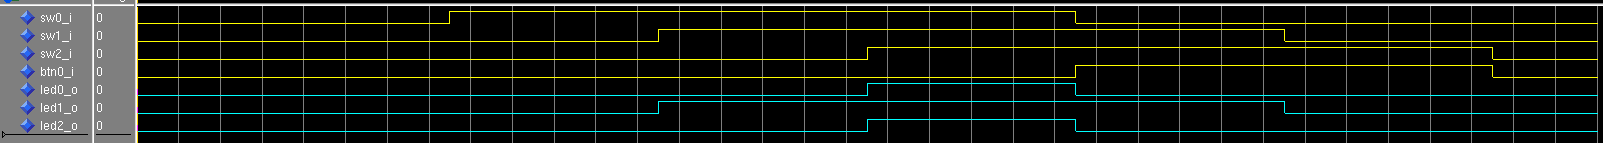
\includegraphics[width=0.98\textwidth]{../Daten/gates.png}
	\caption{Simulation von gates.vhd}
	\label{img_gates}
\end{figure}

In Abb. \ref{img_gates} wurde diese VHDL Datei simuliert.
Man sieht das die gewünschte Funktionalität gegeben ist:
\begin{itemize}
    \item LED $0$ ist nur an wenn alle Schalter an sind
    \item LED $1$ ist an solange mindestens zwei Schalter an sind
    \item LED $2$ ist an wenn Schalter $2$ an und der Knopf nicht gedrückt ist
\end{itemize}

Wir haben diese VHDL-Datei außerdem synthetisiert und dem FPGA aufgespielt um die Funktionalität zu überprüfen.
Es funktionierte einwandfrei.
Ein Bild von einer beispielhaften Schalterstellung ist in Abb. \ref{photo_gates} zu sehen.

\begin{figure}[ht]
	\centering
    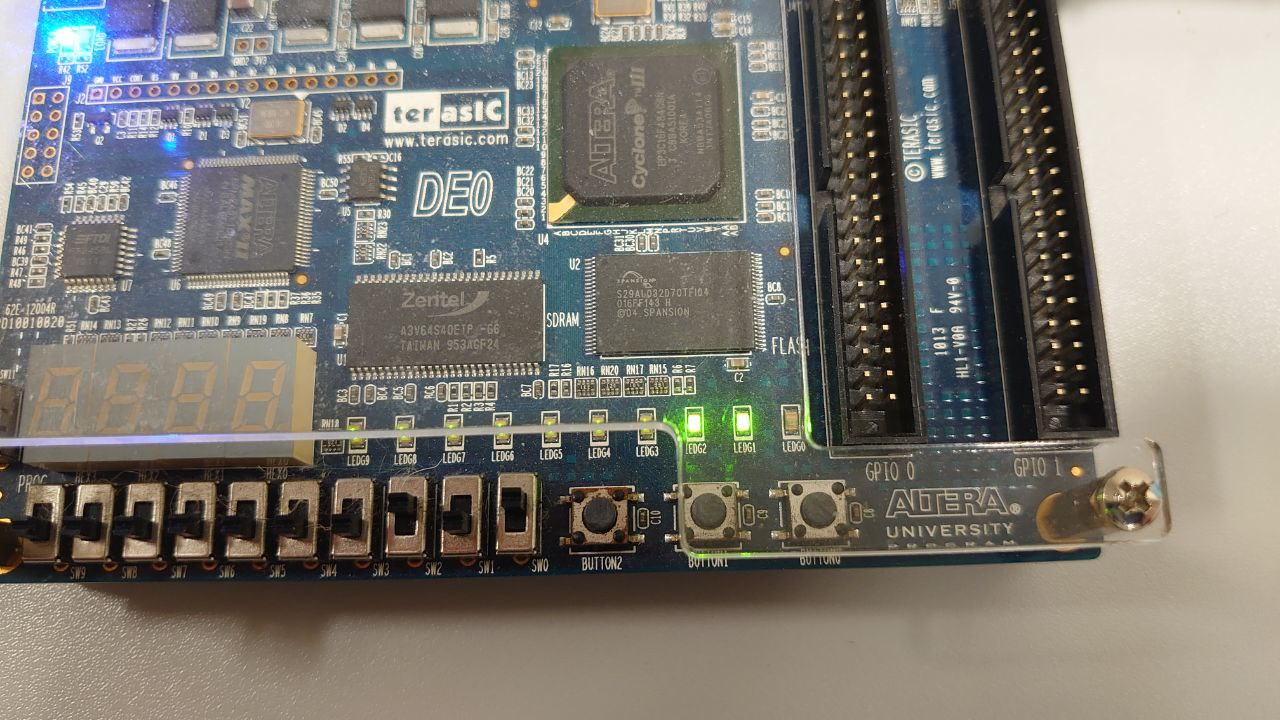
\includegraphics[width=0.98\textwidth]{../Daten/Photo_FPGA_gates.png}
	\caption{Photo des FPGA mit aufgespielter synthetisierter Verknüpfung von gates.vhd in beispielhafter Schalterstellung. Da nur Schalter $0$ und $2$ an (und der Knopf nicht gedrückt) sind sollten LED $1$ und $2$ an sein, und sie sind es.}
	\label{photo_gates}
\end{figure}

\subsection{Modul 1 - \textit{LoHi Detect}}

Ab hier wurde an dem Projekt für die Datenverarbeitung am ATLAS Kalorimeter gearbeitet.
In solchen Anwendungen wird üblicherweise mit einer \textit{Clock}, einem Taktsignal gearbeitet.
Da wir hier mit vorgefertigten Daten arbeiten müssen wir ein Startsignal zum Senden der Daten von außerhalb (vom PC) geben.
Dafür verwenden wir einen Knopf.
Um das Senden der Daten nur einmal und in definierter Weise auszulösen müssen wir den Knopfdruck an die Clock koppeln.
Dafür ist das Modul \textit{LoHi Detect} zuständig.
Die Aufgabe bestand darin das ausgehende Signal (sig\_o) dann auf $1$ zu setzen wenn zu einer steigenden Flanke der Clock der Knopf gedrück ist, zur wiederum nächsten steigenden Flanke der Clock sollte es jedoch wieder auf $0$ gesetzt werden.
Im Folgenden ist der Code dieses Moduls zu sehen:

\lstinputlisting[firstline = 10]{../Daten/lohi_detect/lohi_detect.vhd}

Hier wurde ein neues Syntaxelement genutzt: der \textbf{process}.
Dieser tritt innerhalb der \textbf{architecture} auf und wird immer dann ausgeführt wenn eines der Signale die nach dem Schlüsselwort \textbf{process} aufgezählt werden sich ändert.
Im Gegensatz zum Großteil der restlichen VHDL Syntax wird innerhalb eines \textbf{process} sequentiell gearbeitet.
Eine Änderung der Signale findet jedoch erst statt wenn der Prozess beendet ist.
Dadurch sind \textbf{if} Bedingungen und Schleifen möglich.
Intern (beim synthetisieren) werden diese jedoch aufgedröselt, denn im FPGA läuft nichts tatsächlich sequentiell ab.
In dem Code-Beispiel wird also zu jeder steigenden Flanke der Clock dem Ausgangssignal der Wert des Knopfes AND verknüpft mit dem inversen des internen Signal reg zugewiesen.
Dies ist zum ersten Clock-Zyklus eine $1$.
Dem interne Signal reg wiederum wird der Wert des Eingangssignals zugewiesen.
Das verhindert das im nächsten Clock-Zyklus das Eingangssignal auf das Ausgangssignal übergeht; Statdessen wird das Ausgangssignal $0$.
Solange der Knopf gedrück bleibt ändert sich daran nichts.
Wird der Knopf losgelassen wird zur nächsten steigenden Flanke der Clock das interne Signal auf $0$ gesetzt und man befindet sich im Ausgangszustand.

\begin{figure}[ht]
	\centering
    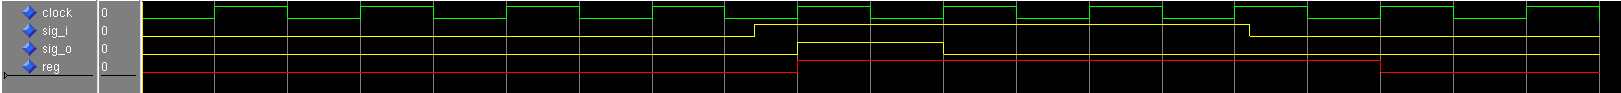
\includegraphics[width=0.98\textwidth]{../Daten/lohi_detect.png}
	\caption{Simulation von lohi\_detect.vhd}
	\label{img_lohi_detect}
\end{figure}

In Abb. \ref{img_lohi_detect} wurde dieses Modul simuliert.
Man sieht das nach Betätigung des Knopfes zur nächsten steigenden Flanke der Clock der Ausgang einen Zyklus lang auf $1$ steht.
Als der Knopf losgelassen wird und das Eingangssignal wieder auf $0$ fällt wird zur nächsten steigenden Flanke der Clock auch das interne Signal reg zurückgesetzt.
